\documentclass[a4paper, oneside]{article}
\special{pdf:minorversion 6}

\usepackage[english, russian]{babel}

\usepackage{fontspec}
\setmainfont[
  Ligatures=TeX,
  Extension=.otf,
  BoldFont=cmunbx,
  ItalicFont=cmunti,
  BoldItalicFont=cmunbi,
]{cmunrm}
\usepackage{unicode-math}

\usepackage[bookmarks=false]{hyperref}
\hypersetup{pdfstartview={FitH},
            pdfauthor={Павел Соболев}}

\usepackage{calrsfs}
\DeclareMathAlphabet{\pazocal}{OMS}{zplm}{m}{n}

\usepackage[table]{xcolor}
\usepackage{booktabs}
\usepackage{caption}

\usepackage{graphicx}
\graphicspath{ {../plots/} }

\usepackage{sectsty}
\sectionfont{\centering}
\subsubsectionfont{\centering\normalfont\itshape}

\newcommand{\npar}{\par\vspace{\baselineskip}}
\newcommand{\su}{\vspace{-0.5em}}
\newcommand{\sd}{\vspace{0.5em}}

\setlength{\parindent}{0pt}

\hypersetup{pdftitle={Специальный практикум (V курс, осень 2021)}}

\begin{document}

\subsubsection*{Специальный практикум (V курс, осень 2021)}
\section*{Разложение бимодальной функции распределения на две нормальные составляющие методом наибольшего правдоподобия}
\subsubsection*{Руководитель: И. И. Никифоров \hspace{2em} Выполнил: П. Л. Соболев}

\vspace{3em}

\subsection*{Задачи}

\begin{itemize}
  \setlength\itemsep{-0.1em}
  \item Определить точечные оценки и доверительные интервалы каждого из параметров модели;
  \item Построить графики профилей каждого из параметров с отмеченными на них доверительными интервалами;
  \item Построить график сравнения наблюдаемого распределения с модельным.
\end{itemize}

\subsection*{Ход выполнения и результаты}

Дифференциальный закон распределения:

$$
\varphi(f) = \frac{c}{\sqrt{2 \pi} \sigma_1} e^{\displaystyle -\frac{(f - \mu_1)^2}{2 \sigma_1^2}} + \frac{1 - c}{\sqrt{2 \pi} \sigma_2} e^{\displaystyle -\frac{(f - \mu_2)^2}{2 \sigma_2^2}}.
$$
\sd

Функция правдоподобия:

$$
L(f_1, f_2, \ldots, f_N; \mu_1, \sigma_1, \mu_2, \sigma_2, c) = \prod_{i=1}^{N} \varphi(f_i; \mu_1, \sigma_1, \mu_2, \sigma_2, c).
$$

Логарифмическая функция правдоподобия:

\su\su
\begin{gather*}
\pazocal{L} = - \sum_{i=1}^{N} \ln \varphi(f_i; \mu_1, \sigma_1, \mu_2, \sigma_2, c) = \\
= \frac{N}{2} \ln (2 \pi) - \sum_{i=1}^{N} \ln \left[ \frac{c}{\sigma_1} e^{\displaystyle -\frac{(f_i - \mu_1)^2}{2 \sigma_1^2}} + \frac{1 - c}{\sigma_2} e^{\displaystyle -\frac{(f_i - \mu_2)^2}{2 \sigma_2^2}} \right] = \\
= \pazocal{L}^{(0)} + \pazocal{L}^{(1)}(f_1, f_2, \ldots, f_N; \mu_1, \sigma_1, \mu_2, \sigma_2, c).
\end{gather*}

Точечные оценки параметров $ \mu_1, \sigma_1, \mu_2, \sigma_2, c $ находятся минимизацией:

$$
\pazocal{L}^{(1)}(\mathbf{f}; \mu_1, \sigma_1, \mu_2, \sigma_2, c) \rightarrow \min, \hspace{2em} \sigma_1, \sigma_2 > 0, \; 0 < c < 1.
$$

\newpage

Результаты минимизации:

\begin{table}[h]
  \centering
  \caption{Точечные оценки и доверительные интервалы параметров}
  \begin{tabular}{cccc}
    \toprule
    Параметр &
    Значение &
    $ \sigma^{-} $ &
    $ \sigma^{+} $ \\
    \midrule
    $ \mu_1 $ & -1.5162 & 0.0550 & 0.0592 \\
    \arrayrulecolor{black!40}
    \midrule
    $ \sigma_1 $ & 0.3948 & 0.0388 & 0.0456 \\
    \midrule
    $ \mu_2 $ & -0.5195 & 0.0717 & 0.0589 \\
    \midrule
    $ \sigma_2 $ & 0.2291 & 0.0364 & 0.0509 \\
    \midrule
    $ c $ & 0.7502 & 0.0591 & 0.0549 \\
    \arrayrulecolor{black}
    \bottomrule
  \end{tabular}
\end{table}

\begin{figure}[h!]
  \centering
  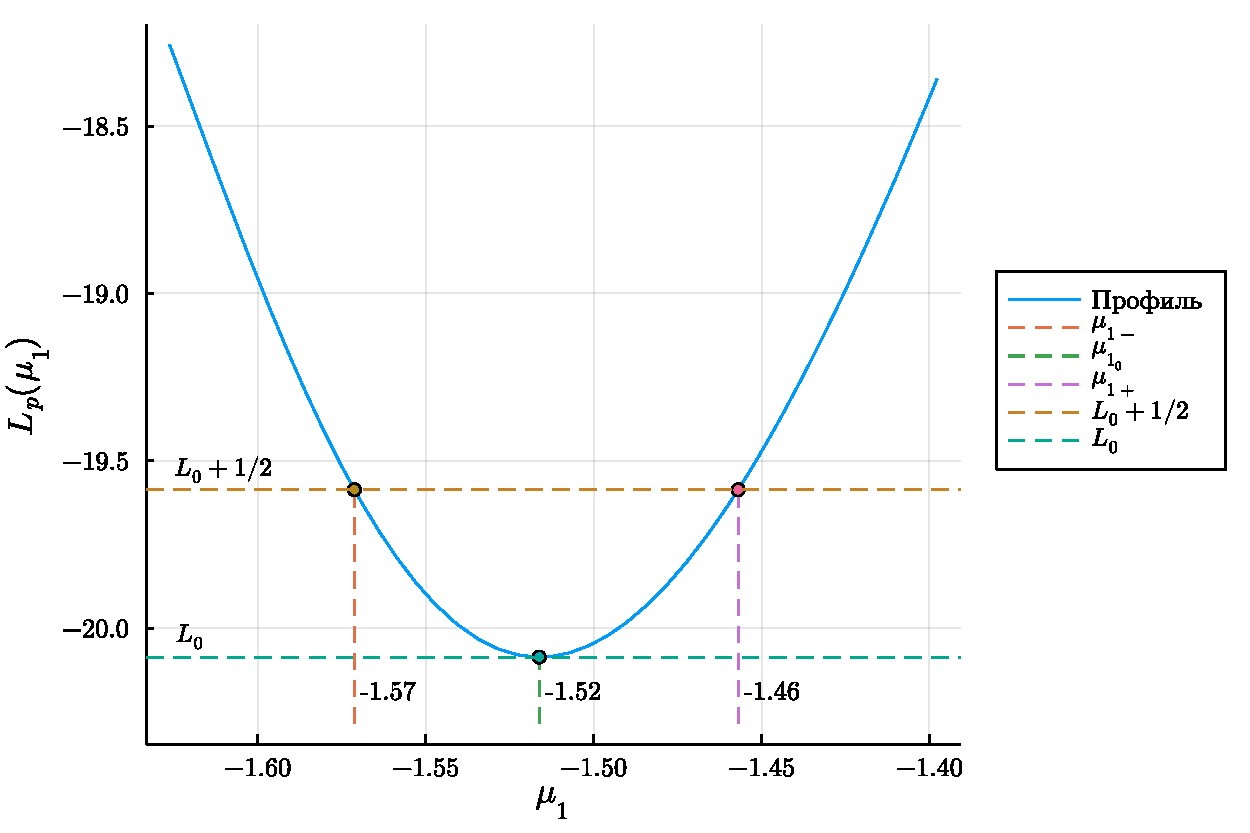
\includegraphics[scale=0.5]{μ₁}
  \caption{Профиль параметра $ \mu_1 $}
\end{figure}

\newpage

\begin{figure}[h!]
  \centering
  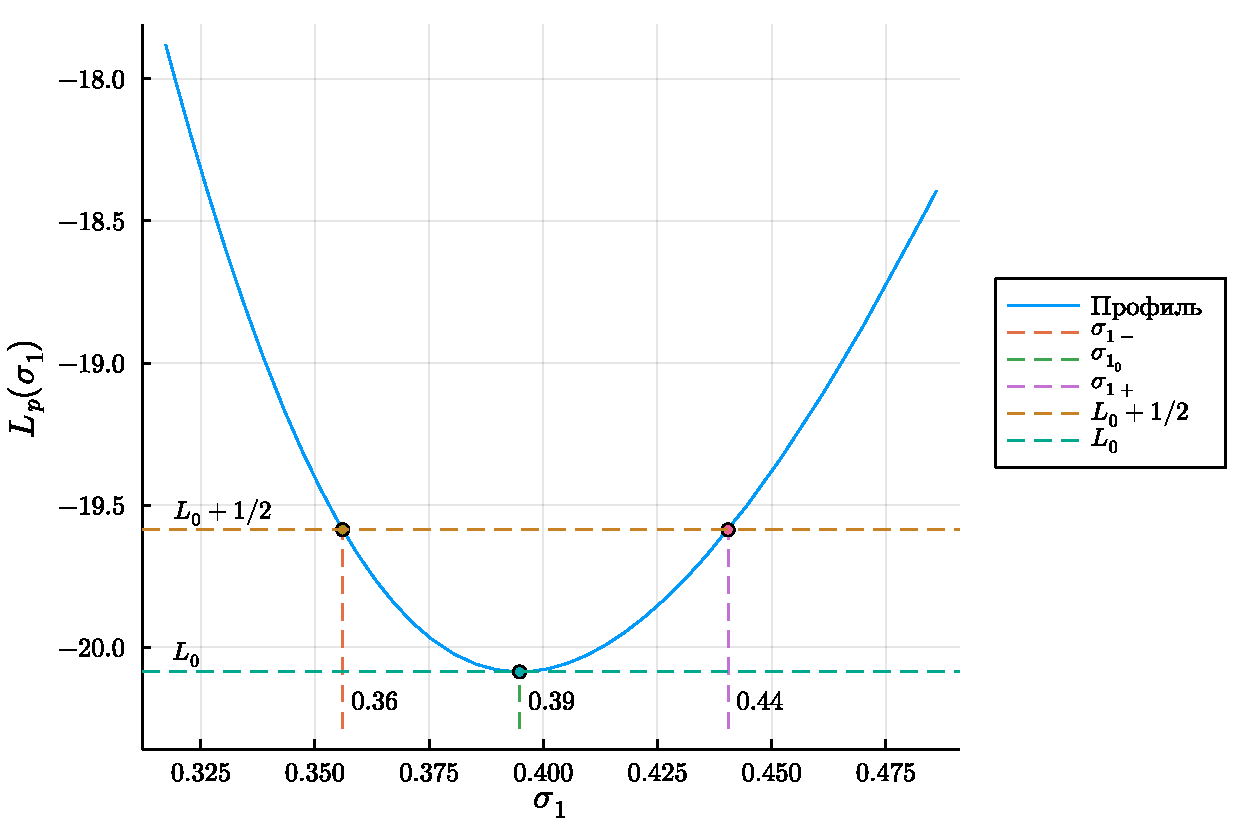
\includegraphics[scale=0.5]{σ₁}
  \caption{Профиль параметра $ \sigma_1 $}
\end{figure}

\begin{figure}[h!]
  \centering
  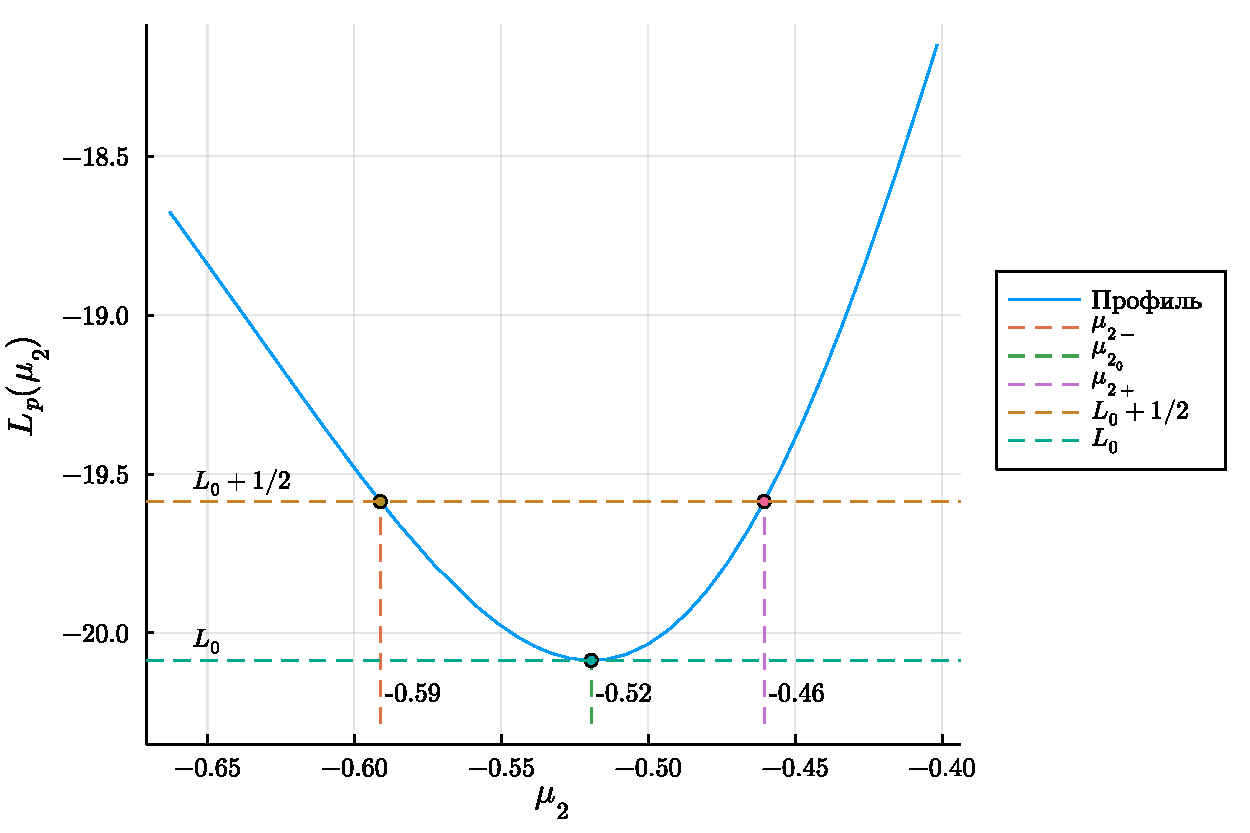
\includegraphics[scale=0.5]{μ₂}
  \caption{Профиль параметра $ \mu_2 $}
\end{figure}

\newpage

\begin{figure}[h!]
  \centering
  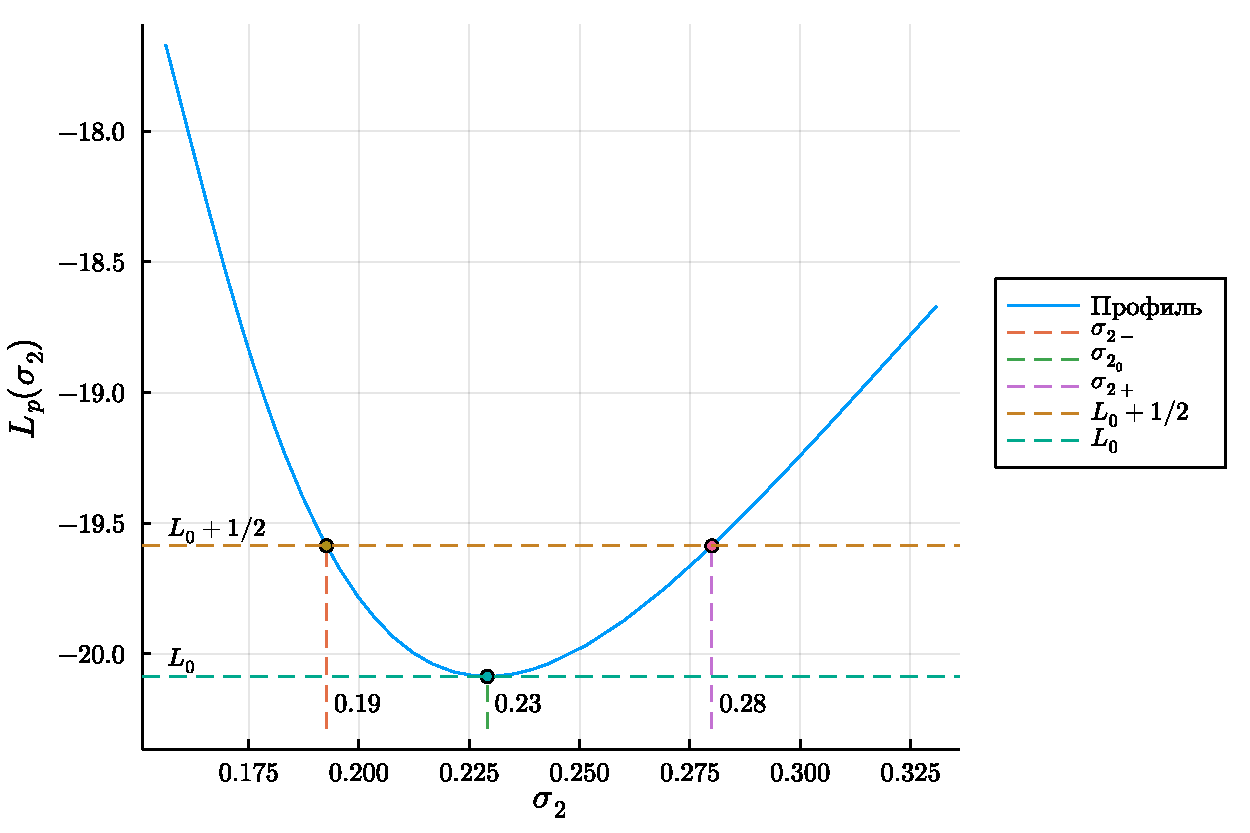
\includegraphics[scale=0.5]{σ₂}
  \caption{Профиль параметра $ \sigma_2 $}
\end{figure}

\begin{figure}[h!]
  \centering
  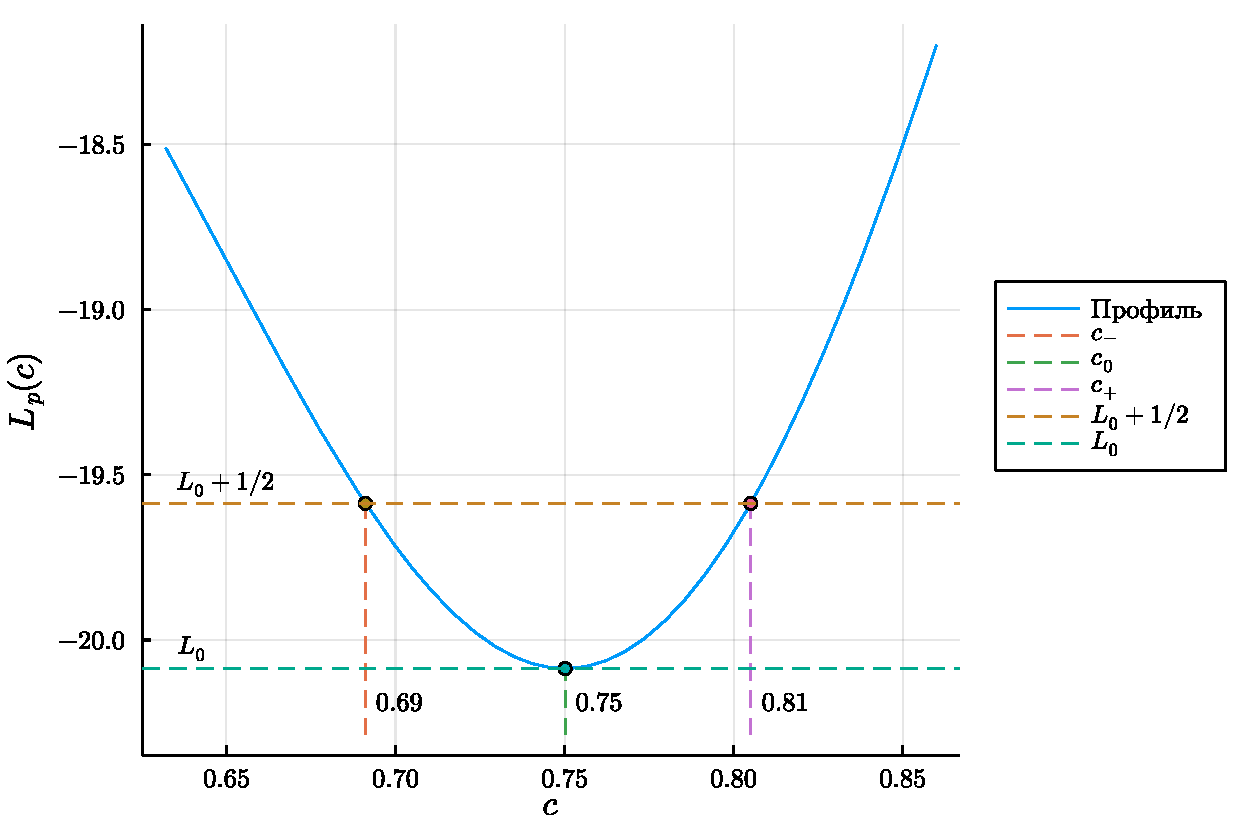
\includegraphics[scale=0.5]{c}
  \caption{Профиль параметра $ c $}
\end{figure}

\newpage

\begin{figure}[h!]
  \centering
  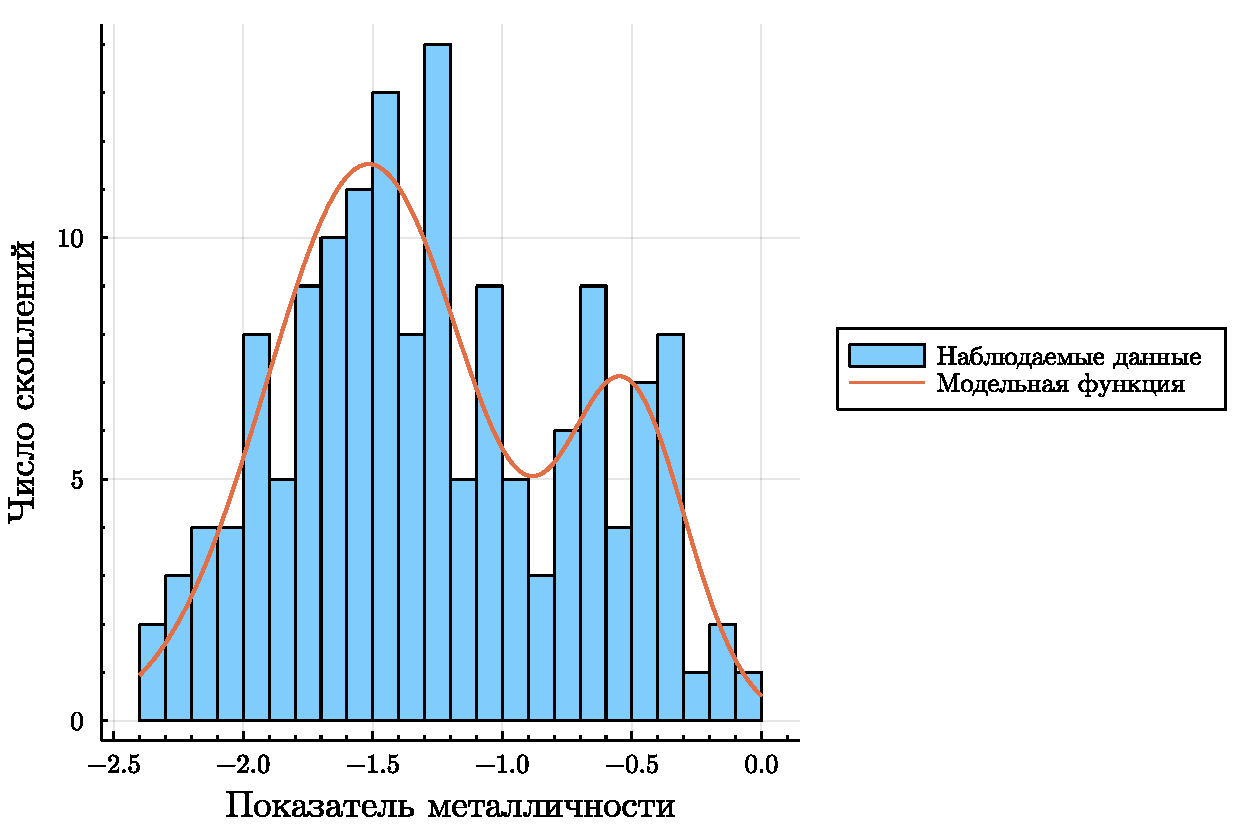
\includegraphics[scale=0.5]{histogram}
  \caption{Модельная функция и гистограмма \\ наблюдаемого распределения}
\end{figure}

\end{document}